% Chapter Template

\chapter{Ensayos y resultados} % Main chapter title

\label{Chapter4} % Change X to a consecutive number; for referencing this chapter elsewhere, use \ref{ChapterX}
Todos los capítulos deben comenzar con un breve párrafo introductorio que indique cuál es el contenido que se encontrará al leerlo.  La redacción sobre el contenido de la memoria debe hacerse en presente y todo lo referido al proyecto en pasado, siempre de modo impersonal.

%----------------------------------------------------------------------------------------
%	SECTION 1
%----------------------------------------------------------------------------------------

\section{Verificaciones funcionales del hardware}

\subsection{Verificación del proceso de ingesta en tiempo real MQTT}


\begin{center}
   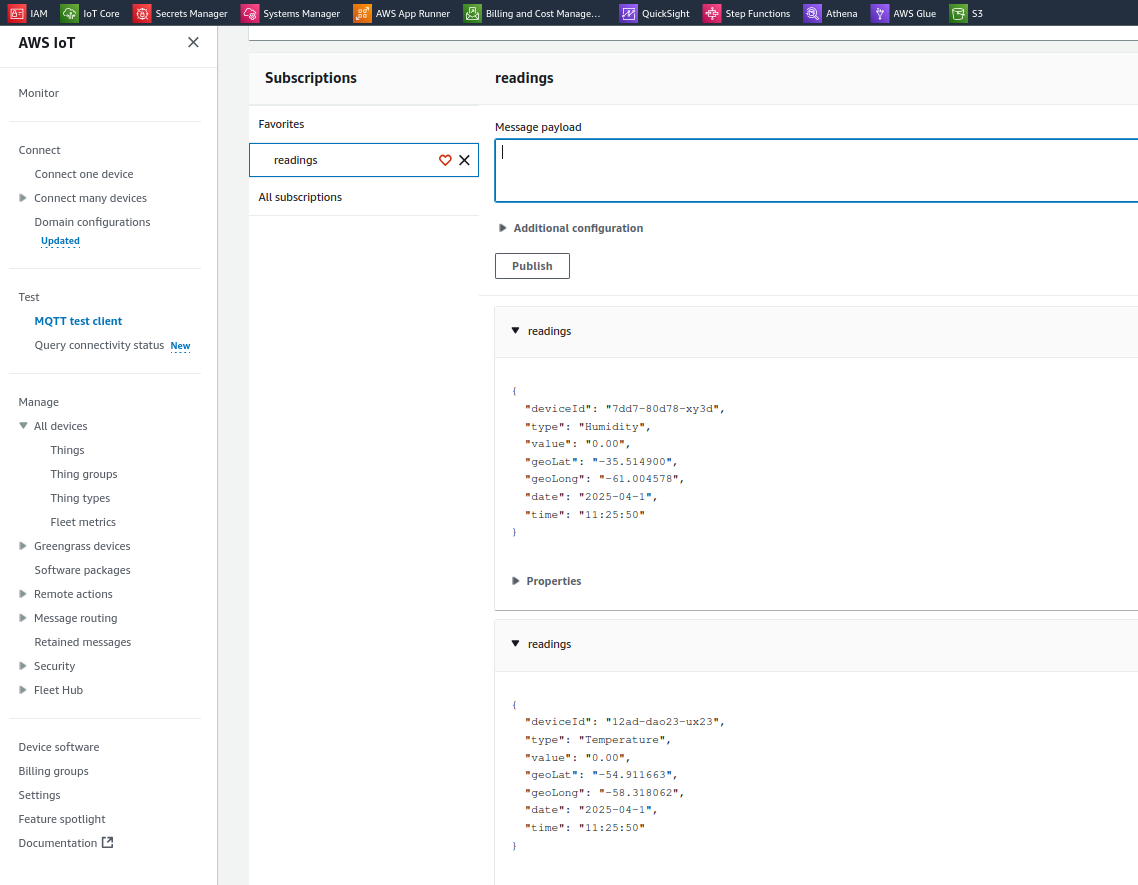
\includegraphics[scale=0.35]{AWS/aws_iot_core_mqtt_test_2}
   \captionof{figure}{Prueba de recepción de mensajes MQTT.}
   \label{fig:aws_iot_core_mqtt_test_2}
\end{center}

\subsection{Verificación del proceso de distribución de eventos en AWS}


\begin{center}
   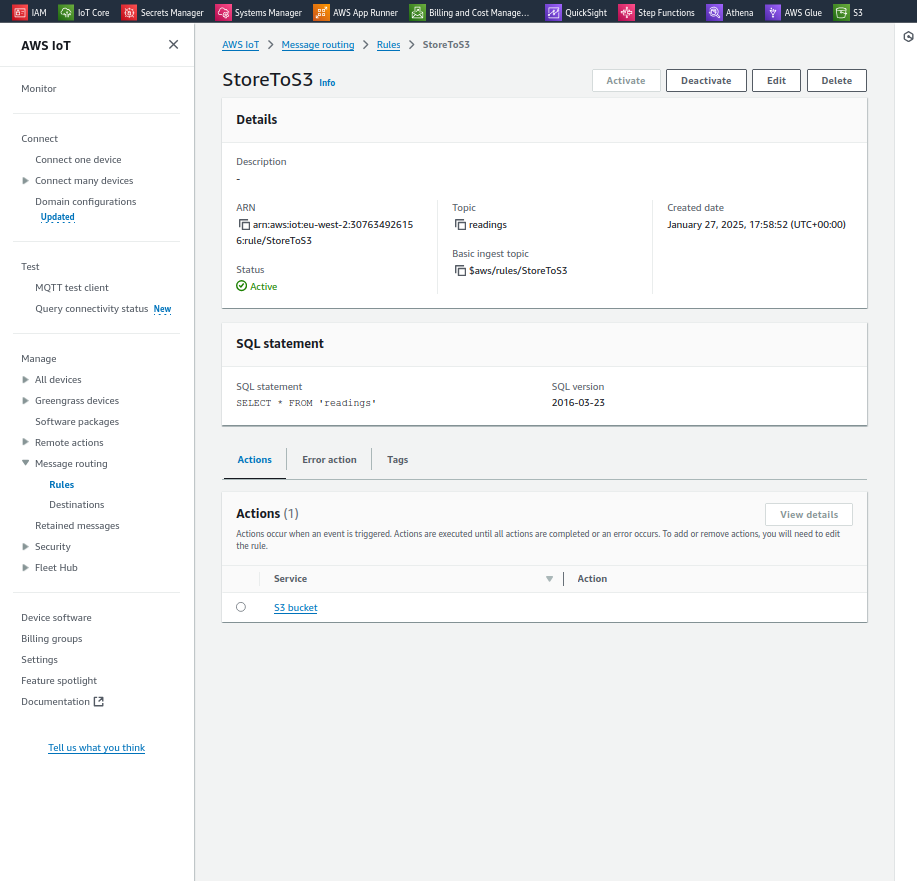
\includegraphics[scale=0.4]{AWS/aws_iot_core_message_routing}
   \captionof{figure}{Configuración de redirección de mensajes MQTT.}
   \label{fig:aws_iot_core_message_routing}
\end{center}


\subsection{Verificación de fondos necesarios para realizar despliegues en redes Holesky y Sepolia}


\begin{center}
   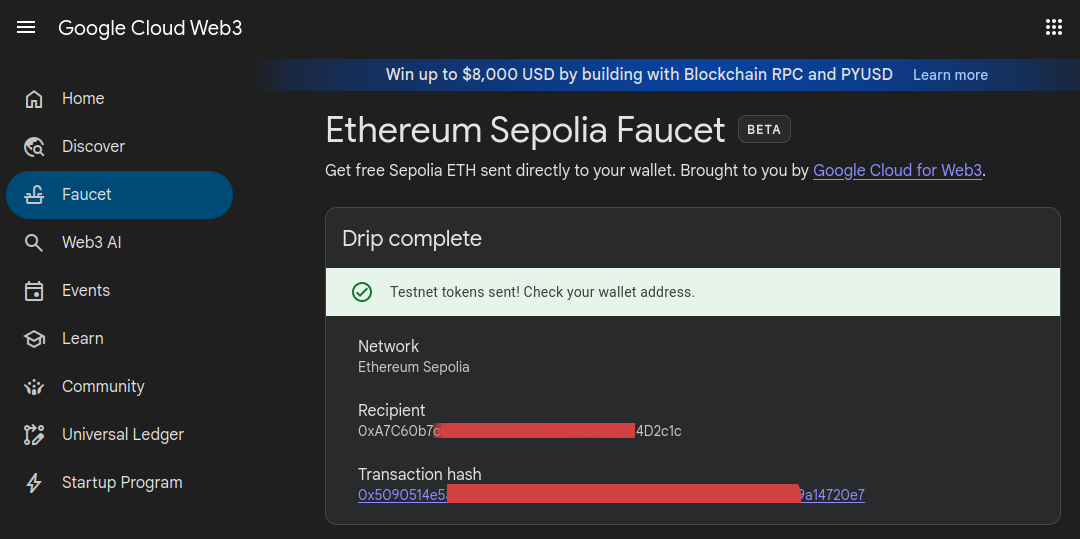
\includegraphics[scale=0.35]{blockchain/google_faucets2}
   \captionof{figure}{Obtención de créditos mediante Google Web3.}
   \label{fig:google_faucets2}
\end{center}

\begin{center}
   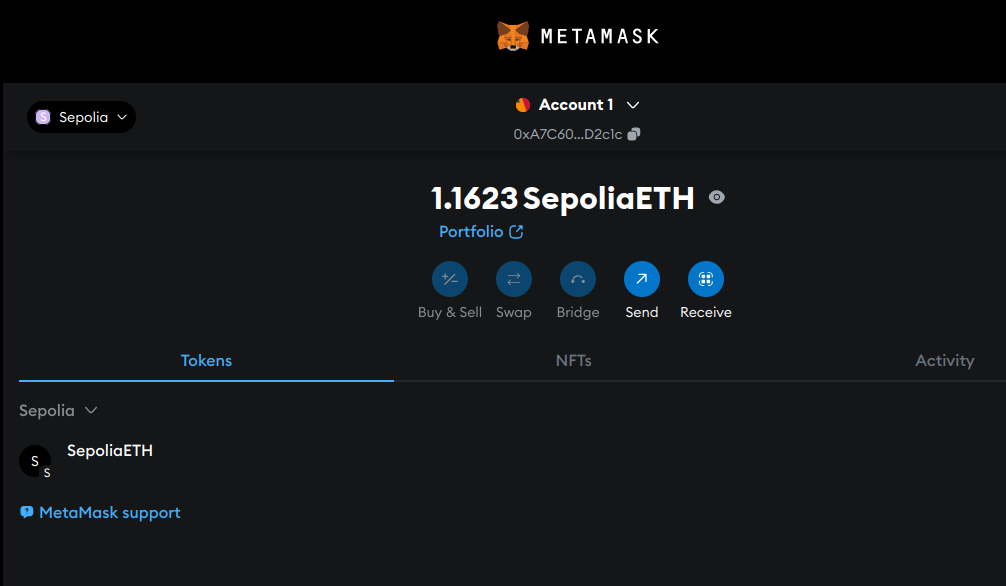
\includegraphics[scale=0.35]{blockchain/metamask_balance}
   \captionof{figure}{Saldo en Metamask.}
   \label{fig:metamask_balance}
\end{center}


\begin{center}
   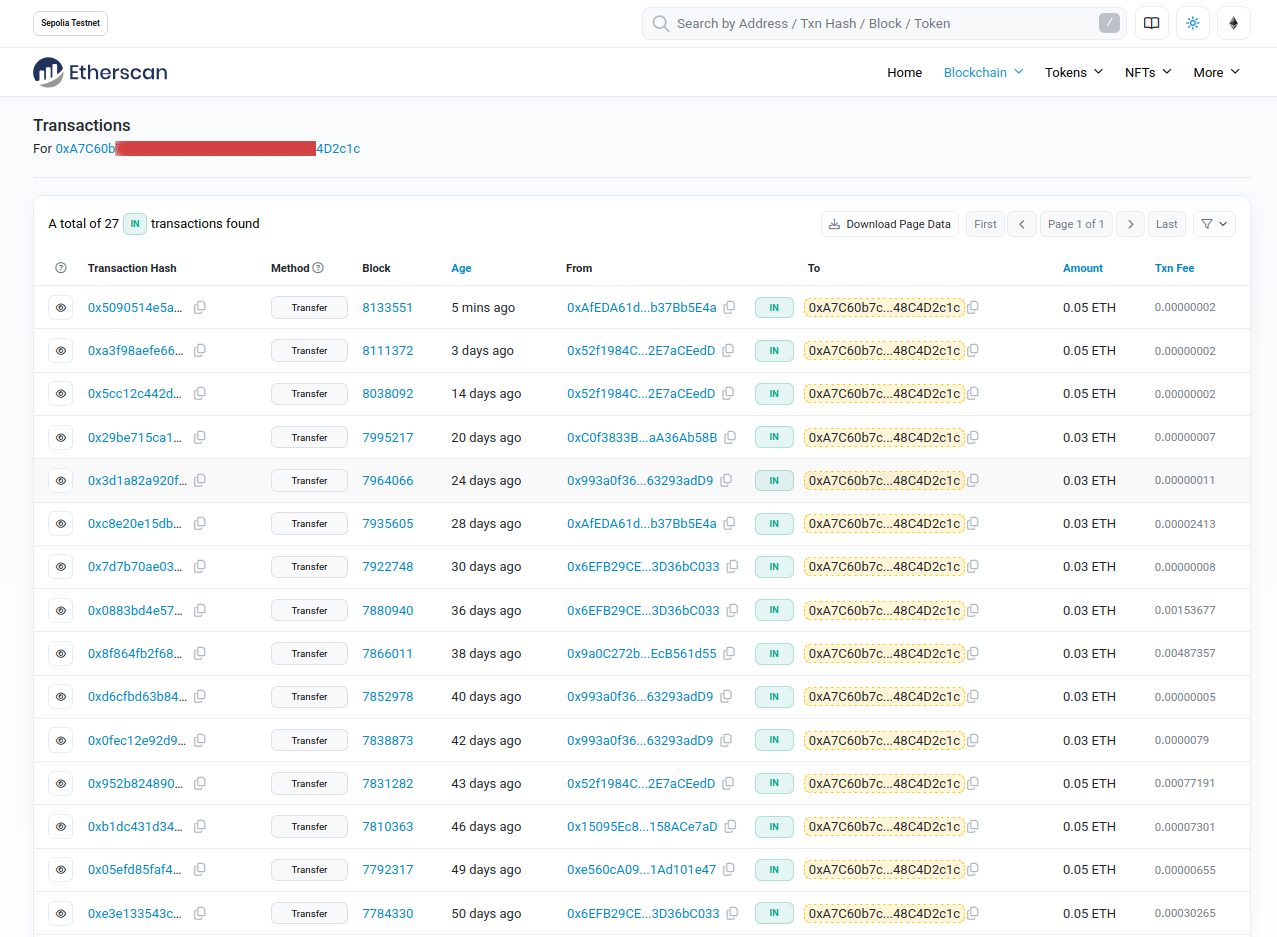
\includegraphics[scale=0.3]{blockchain/sepolia_funding2}
   \captionof{figure}{Transacciones de generación de fondos de prueba.}
   \label{fig:sepolia_funding2}
\end{center}



\begin{center}
   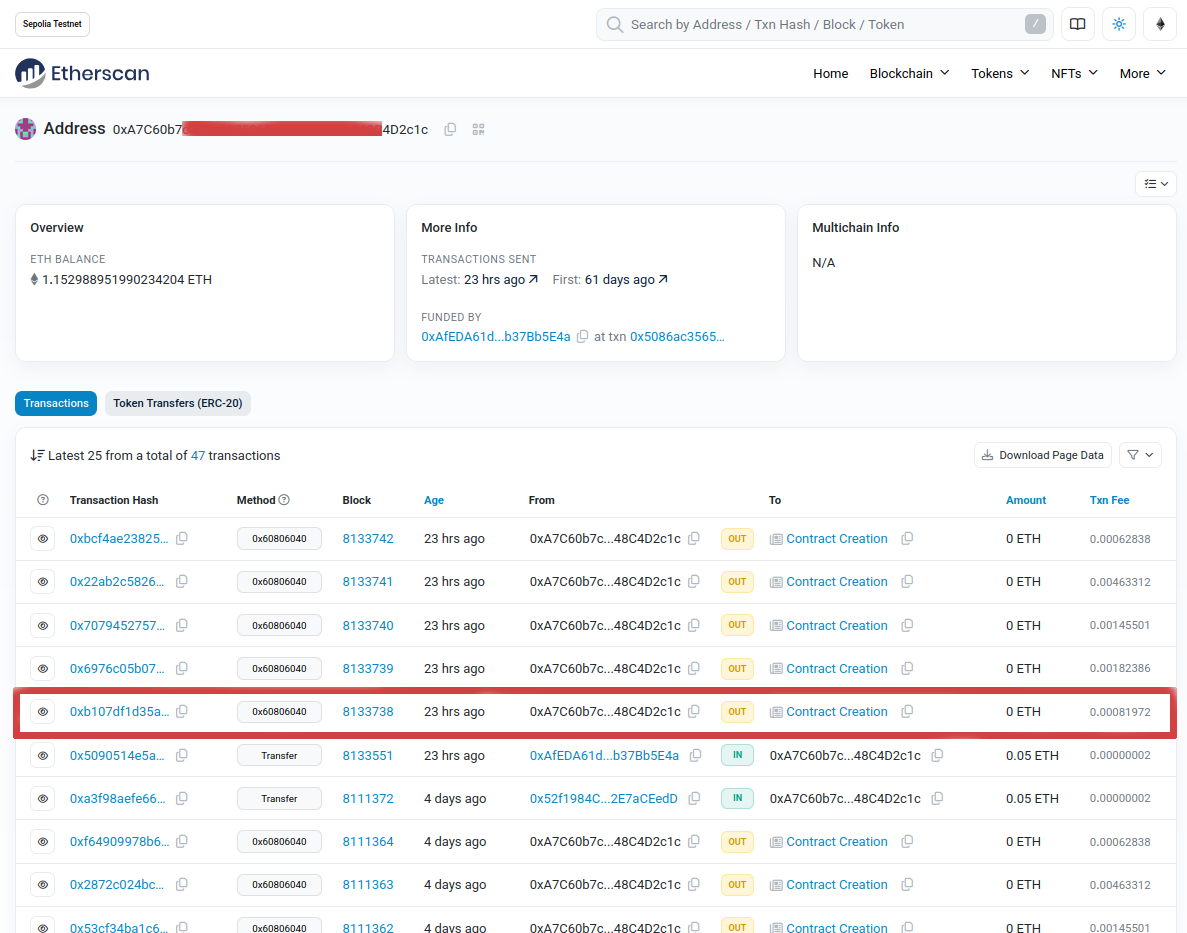
\includegraphics[scale=0.35]{blockchain/sm_deployment_etherscan1}
   \captionof{figure}{Transacciones de despliegue en Sepolia.}
   \label{fig:sm_deployment_etherscan1}
\end{center}

\begin{center}
   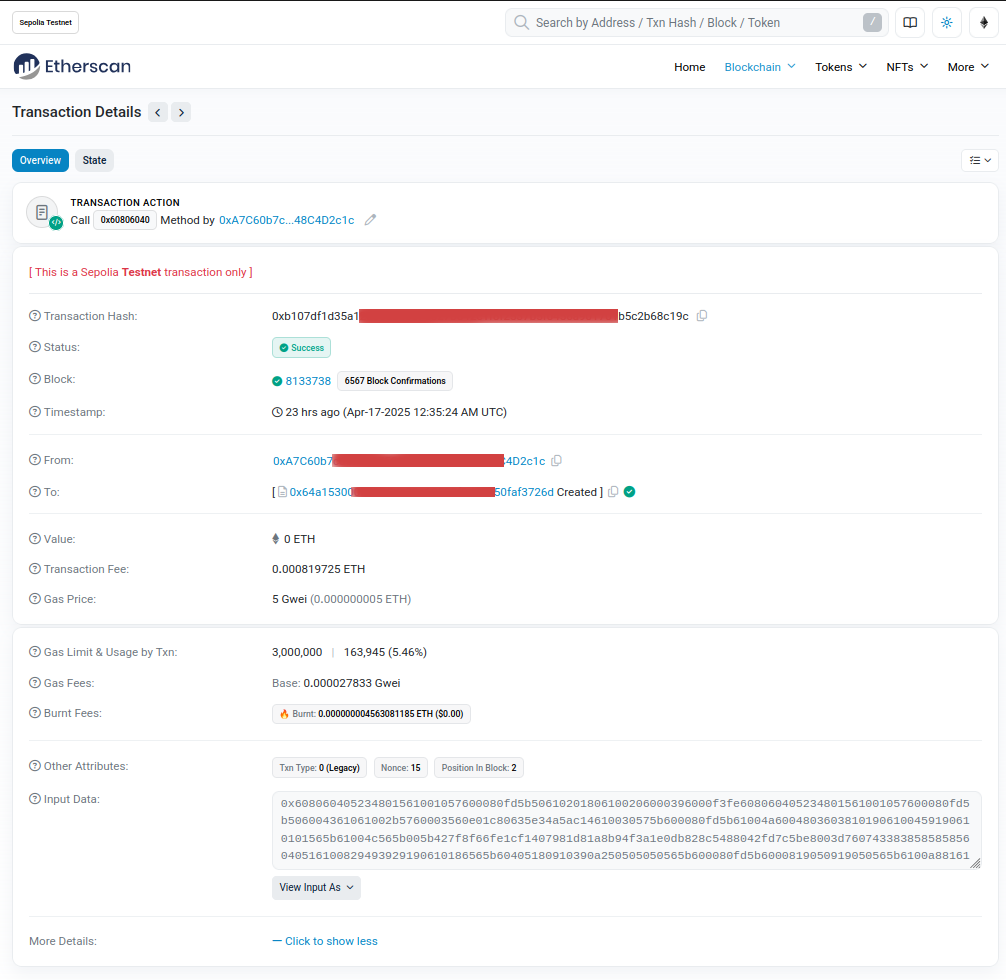
\includegraphics[scale=0.35]{blockchain/sm_deployment_etherscan2}
   \captionof{figure}{Detalles del contrato desplegado en Sepolia.}
   \label{fig:sm_deployment_etherscan2}
\end{center}



\subsection{Verificación del proceso de despliegue de los Smart Contracts}

\begin{center}
   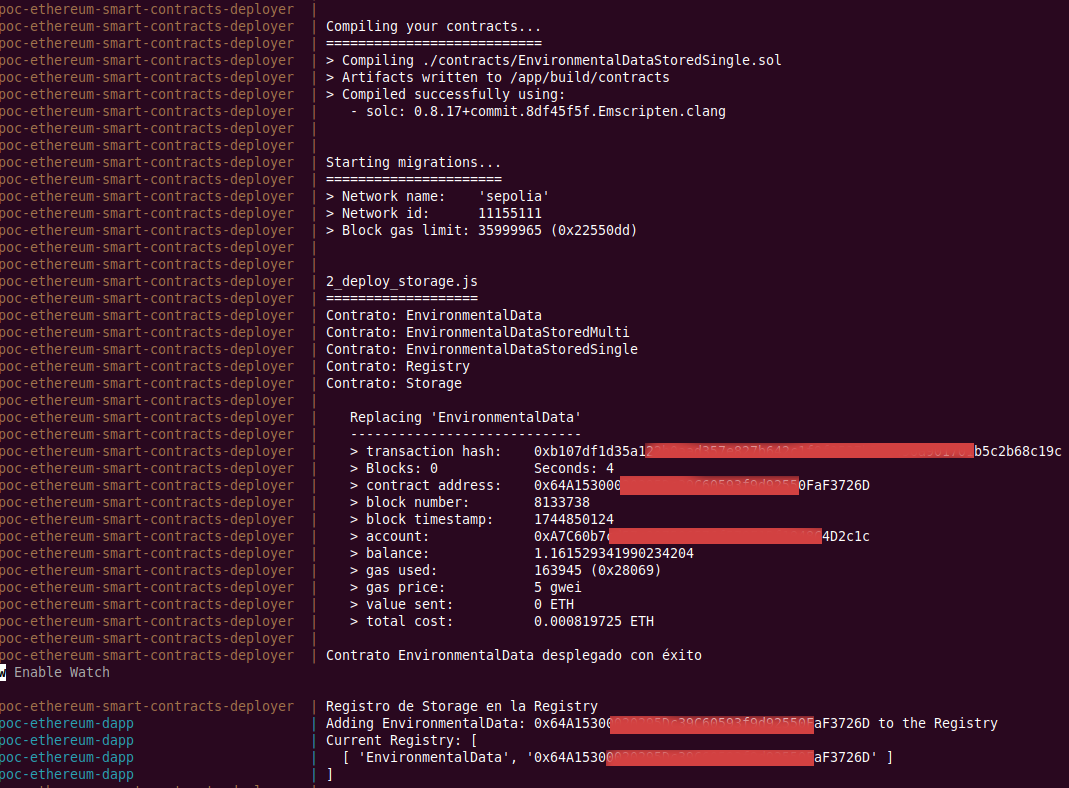
\includegraphics[scale=0.35]{blockchain/sm_deployment}
   \captionof{figure}{Salida por pantalla durante el proceso de despliegue de los componentes blockchain.}
   \label{fig:sm_deployment}
\end{center}


\subsection{Verificación del proceso de despliegue de la dApp}


\begin{center}
   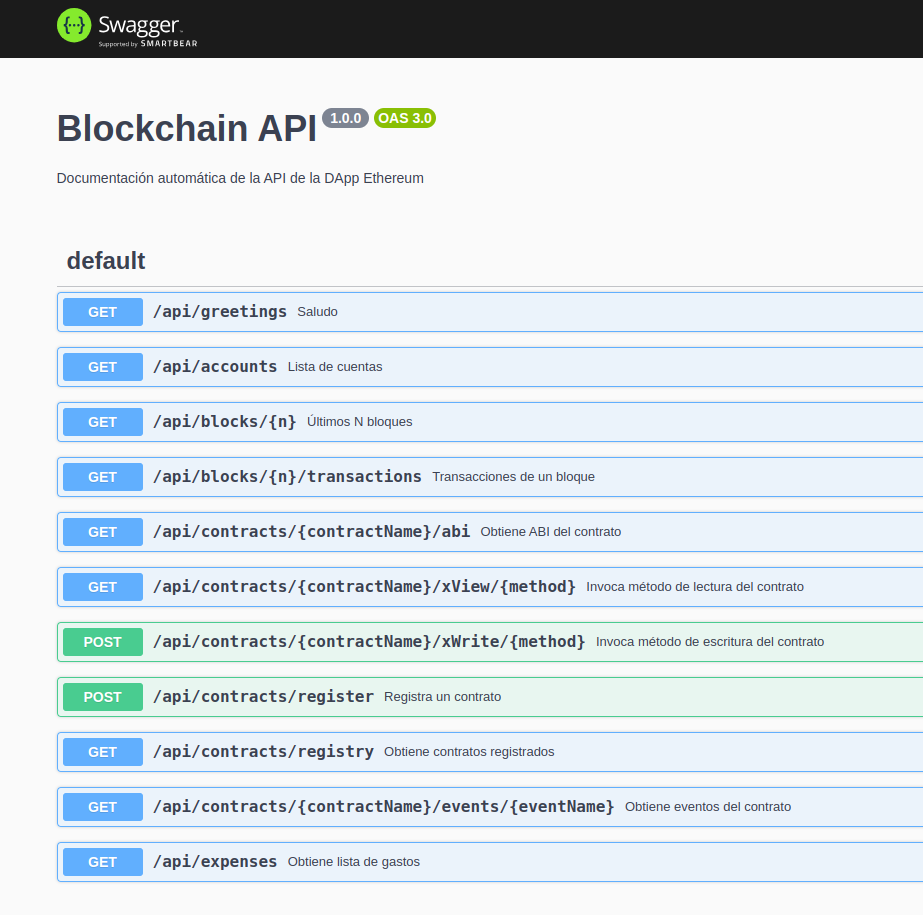
\includegraphics[scale=0.4]{blockchain/dapp_endpoints}
   \captionof{figure}{Endpoints expuestos por la dApp.}
   \label{fig:dapp_endpoints}
\end{center}


\begin{center}
   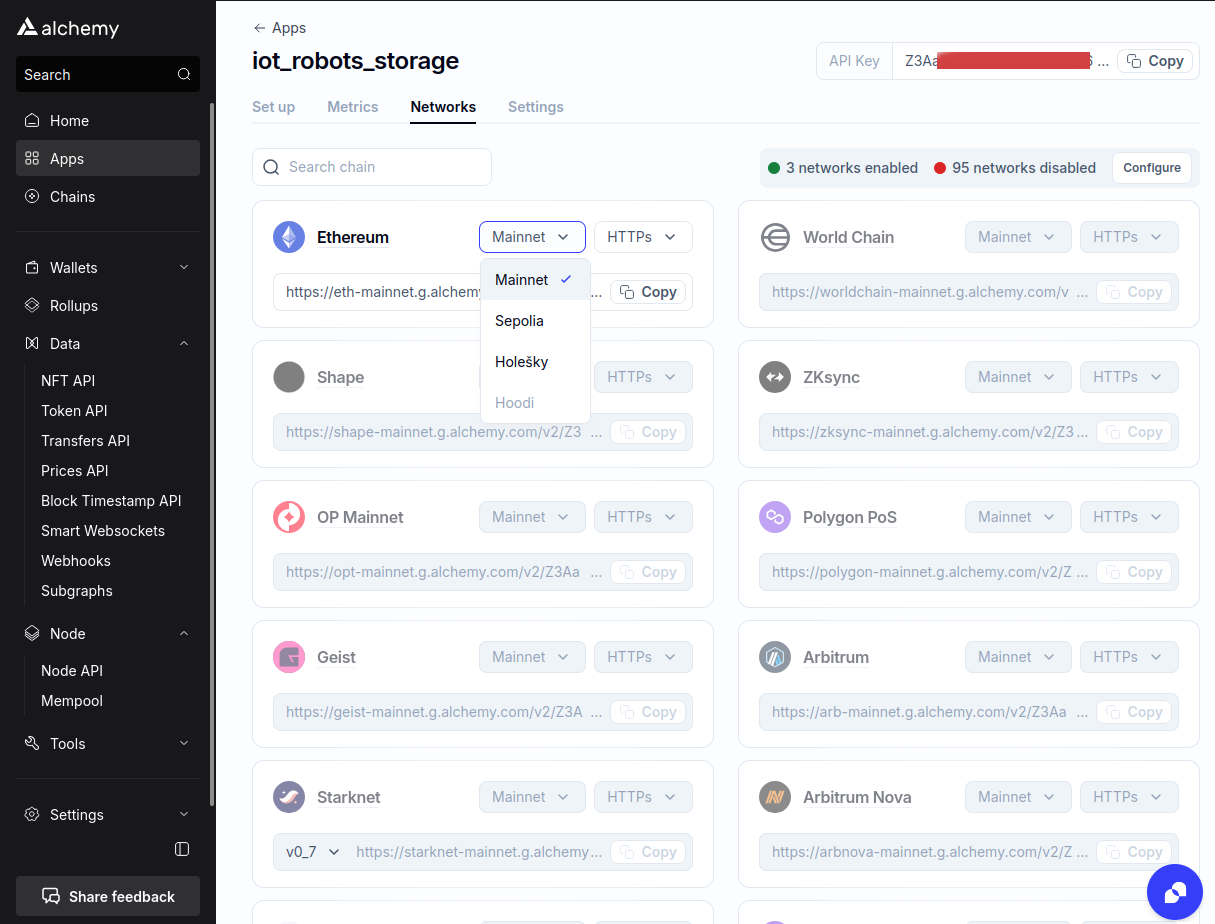
\includegraphics[scale=0.3]{blockchain/alchemy1}
   \captionof{figure}{Frontend the Alchemy.}
   \label{fig:alchemy1}
\end{center}


\subsection{Verificación del proceso de invocación de la dApp}

\subsection{Verificación del proceso de invocación de los Smart Contracts}

\subsection{Validación de los datos almacenados en Ethereum}

\subsection{Verificación del proceso de almacenamiento de readings, transacciones y contracts en AWS S3}


\begin{center}
   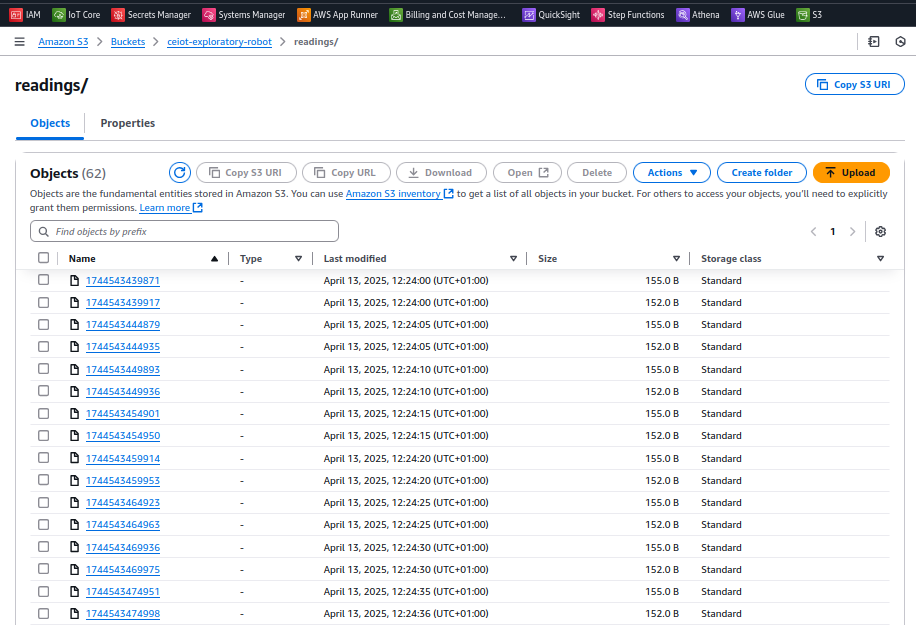
\includegraphics[scale=0.4]{AWS/aws_s3_bucket_data2}
   \captionof{figure}{Almacenamiento de mensajes JSON en AWS S3.}
   \label{fig:aws_s3_bucket_data2}
\end{center}


\begin{center}
   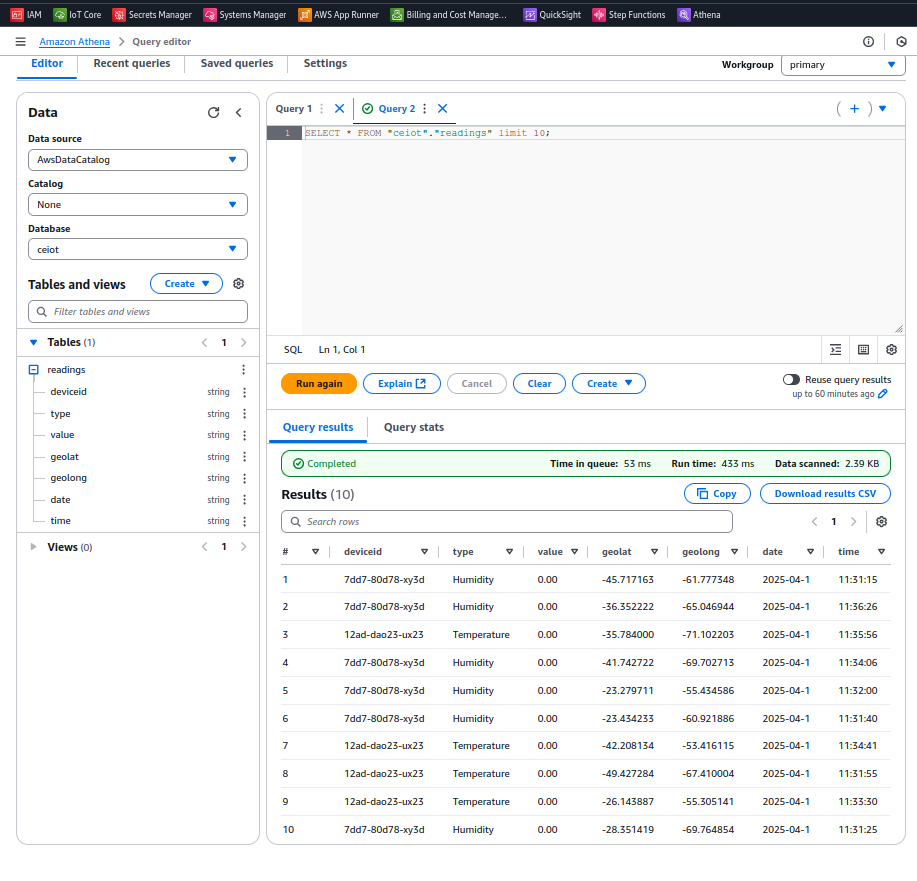
\includegraphics[scale=0.4]{AWS/aws_athena_config}
   \captionof{figure}{Consulta de datos SQL desde AWS Athena.}
   \label{fig:aws_athena_config}
\end{center}



\subsection{Verificación del proceso de ingesta y transformación de datos batch en Fabric}



\begin{center}
   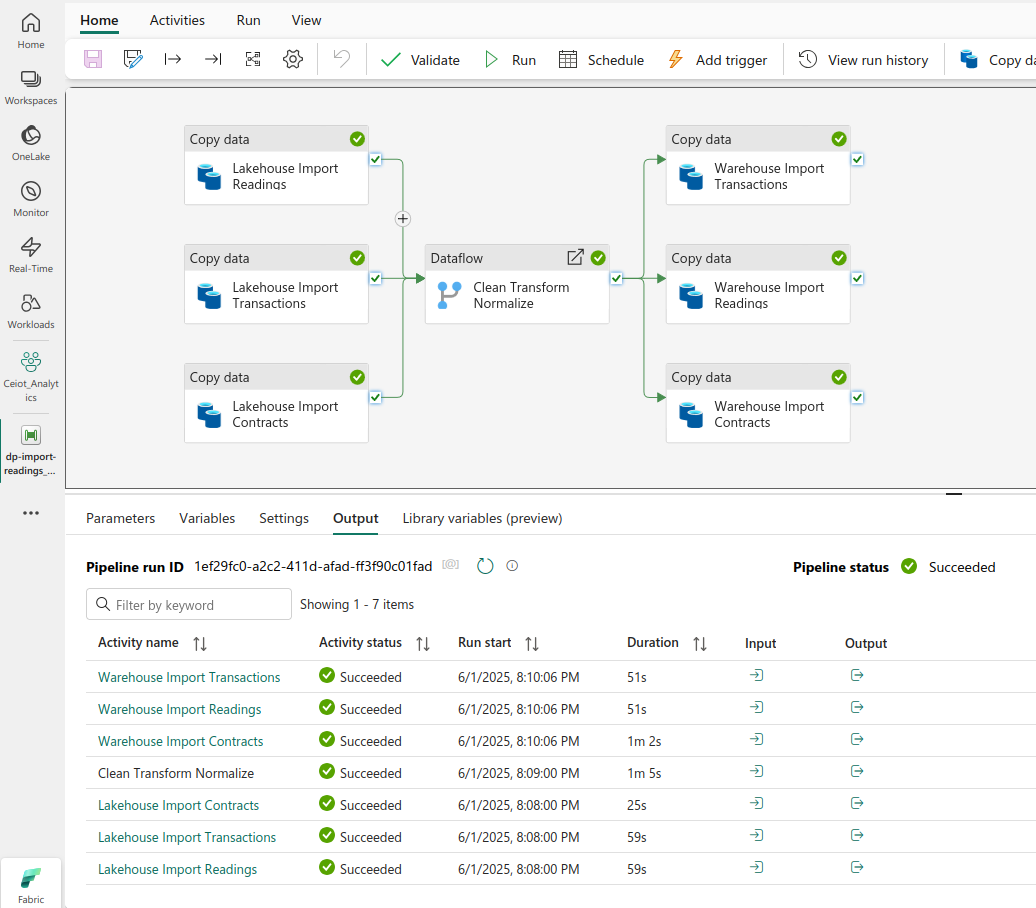
\includegraphics[scale=0.35]{Azure/datafactory_result}
   \captionof{figure}{Correcta ejecución del pipeline punta-a-punta con Azure Data Factory y Dataflows.}
   \label{fig:powerbi1}
\end{center}
 

\subsection{Validación del modelo de datos en el Semantic Model}

\subsection{Validación del reporte final generado en PowerBI}

\begin{center}
   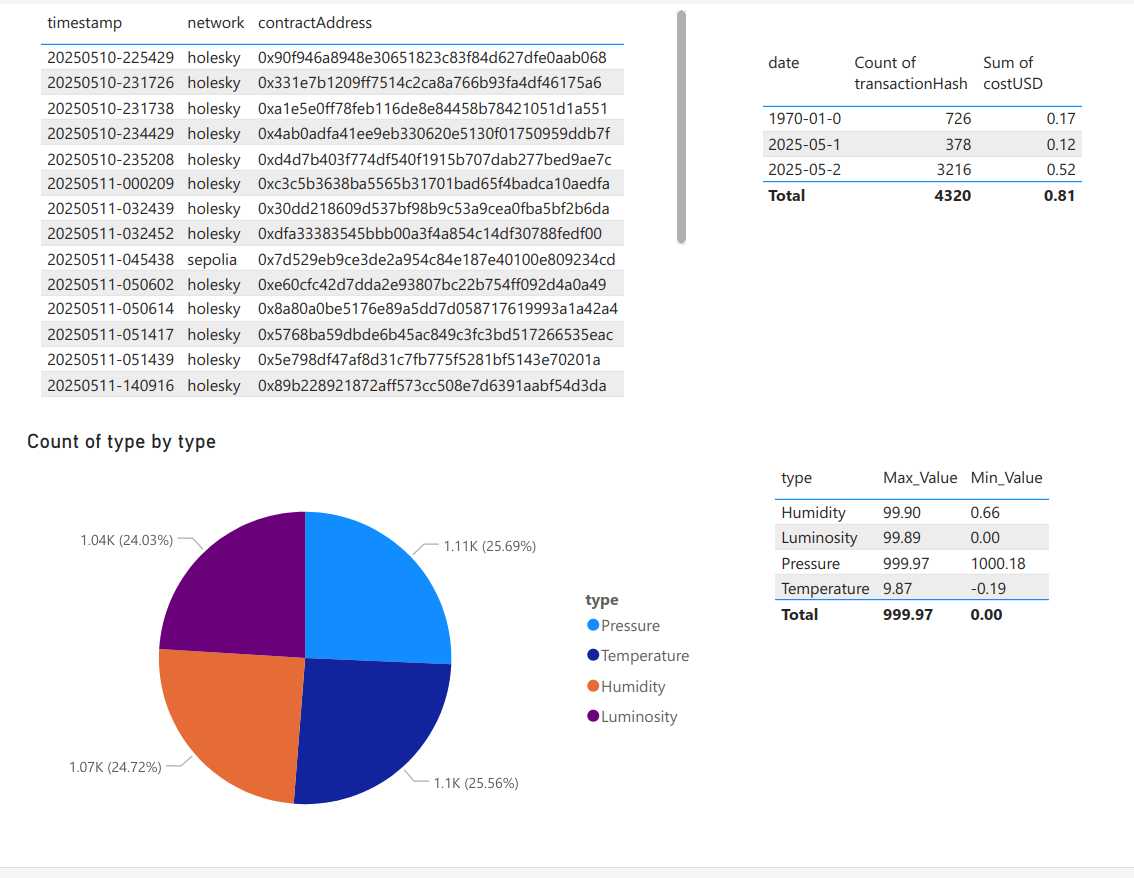
\includegraphics[scale=0.4]{Azure/powerbi}
   \captionof{figure}{Dashboard PowerBI.}
   \label{fig:powerbi1}
\end{center}
 

\section{Pruebas funcionales del hardware}
